\documentclass{lecturefig}
\begin{document}
\begin{frame}[fragile]
  \begin{tikzpicture}[]
    \tikzset{
      mem/.style={font=\ttfamily}
    }
    \def\B#1{\tikz[baseline]\node[mem,anchor=base,inner sep=2pt,onslide=<4->{draw}]{#1};}
    \node[fill=safegreen!20,text width=3.1cm,mem](data){\B{98 52 94 82 72} \B{28 47 85} \B{18 83} \B{58 36} \B{14 89 48}};
    \node[fill=luhblue!20,text width=3.1cm,below=0.2 of data,mem](ops){\alt<-3>{DF 73 94 7E 54 5A \alt<-3>{17 01}{fib()} F9 65 4E EF F9 F7 9E 6F FF FF}{func main() \{\\connect()\\\}}};
    \node[anchor=west,right=0 of data.south east](cpu){
\includegraphics[width=5mm]{fig/07-cpu.png}};
    \draw[->] (ops.east) -| (cpu);
    \draw[<->] (cpu) |- (data.east);
    \node[draw,fit=(data) (ops) (cpu)] {};

    
    \node[fill=safegreen!20,text width=3.1cm,mem, right=5 of data](data2){98 52 94 77 72 28 47 85 18 83 92 58 36 14 89 48 10 21};
    \node[fill=luhblue!20,text width=3.1cm,below=0.2 of data2,mem](ops2){DF 73 94 7E 54 5A 17 01 F9 65 4E EF F9 F7 9E 6F FF FF};
    \node[anchor=west,left=0 of data2.south west](cpu2){
\includegraphics[width=5mm]{fig/07-cpu.png}};
    \draw[->] (ops2.west) -| (cpu2);
    \draw[<->] (cpu2) |- (data2.west);
    \node[draw,fit=(data2) (ops2) (cpu2)] {};

    \node [fill=srared!20,mem] at ($(cpu)!0.5!(cpu2)$) (net) {\alt<-3>{11 22 33 44 87}{TCP SYN}};
    \draw[<->] ($(net.north west)+(up:1ex)$) -- ($(net.north east)+(up:1ex)$);

    \node[above=0.2 of net]{
        \Large \structure{Computer}
      };

    \begin{visible}<2->
      \node[below=2.5cm of net] (brains) {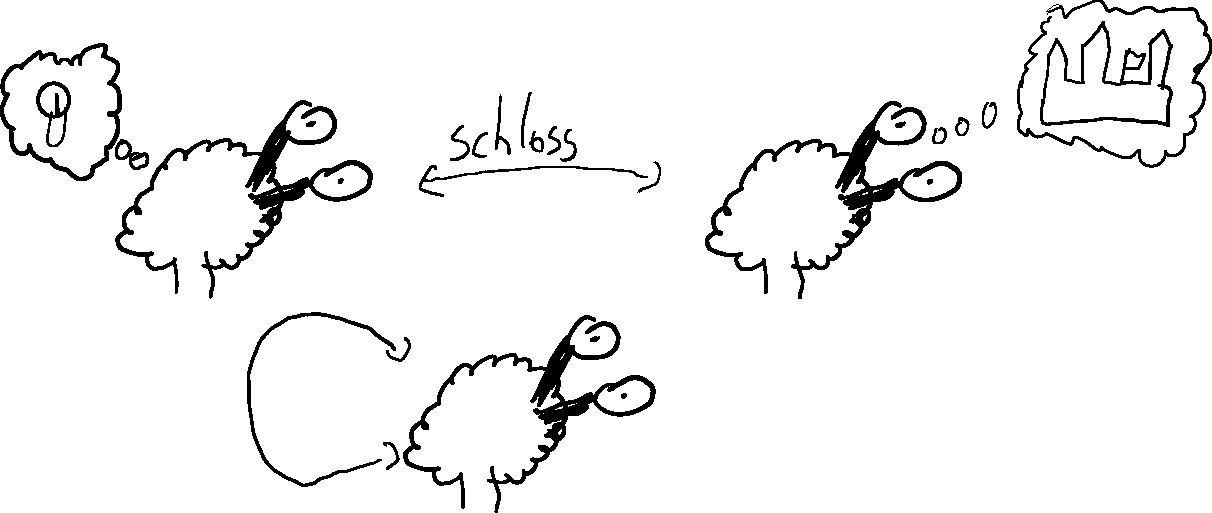
\includegraphics[width=12cm]{fig/11-brains}};
      \draw[thick] (brains.north west) -- (brains.north east);
    \end{visible}
    \begin{visible}<3->
      \node[align=left,anchor=south east] at (brains.south east){
        \begin{minipage}{4.5cm}
          -- Kaum Speicher\\
          -- Kaum Bandbreite\\
          -- Kaum Rechenleistung\\
          -- Uneindeutige Operationen
        \end{minipage}
      };

      \node[align=left,anchor=south west] at (brains.south west){
        \Large \structure{Gehirne}
      };
    \end{visible}
    \begin{visible}<4->
      \node[fill=safegreen!30,draw,align=center] at (brains.north) {Abstraktionen und Strukturen\\ to the Rescue};
    \end{visible}
  \end{tikzpicture}
\end{frame}
\end{document}
